% This is samplepaper.tex, a sample chapter demonstrating the
% LLNCS macro package for Springer Computer Science proceedings;
% Version 2.20 of 2017/10/04
%
\documentclass[runningheads]{llncs}
%
\usepackage{graphicx}
% Used for displaying a sample figure. If possible, figure files should
% be included in EPS format.
%
% If you use the hyperref package, please uncomment the following line
% to display URLs in blue roman font according to Springer's eBook style:
% \renewcommand\UrlFont{\color{blue}\rmfamily}

\begin{document}
%
\title{A Shader-Based Architecture for Virtual Reality Applications on Mobile Devices\thanks{Supported by SIDIA}}
%
%\titlerunning{Abbreviated paper title}
% If the paper title is too long for the running head, you can set
% an abbreviated paper title here
%
\author{Adriano M. Gil \and Thiago S. Figueira}
%
\authorrunning{Adriano Gil \and Thiago Figueira}
% First names are abbreviated in the running head.
% If there are more than two authors, 'et al.' is used.
%
\institute{SIDIA Instituto de Ci\^encia e Tecnologia, Manaus, Brazil
\email{\{adriano.gil,thiago.figueira\}@sidia.com}}
%
\maketitle              % typeset the header of the contribution
%
\begin{abstract}
As new technologies for CPUs and GPUs are released, games showcase improved graphics, physics simulations, and responsiveness. For limited form-factors such as virtual reality head-mounted displays though, it is possible  to explore alternatives components to harness additional performance such as the GPU. This paper introduces a shader-based architecture for developing games using shared resources between the CPU and the GPU.

\keywords{First keyword  \and Second keyword \and Another keyword.}
\end{abstract}
%
%
%
\section{Introduction}

% TODO: Importance of VR
Virtual reality (VR) brings the promise of a revolution in the way entertainment is consumed in present times. The user is placed at the center of the action and perceives content from every direction.

% TODO: Performance issues games
Games, for their part, transport players to a world envisioned by game designers and developers. As the technology for other form factors such as PC and console advances, VR players want life-like graphics and improved responsiveness.

% TODO: Game architectures
Modern mainstream game consoles and PC sets allow parallel computing to be performed. In order to harness this extra computing power, it is necessary to move tasks from the single threaded game loop and place the ones that can run in parallel in different processors.  

% TODO: Reasons/Motivation for a Shader-based architecture
VR devices, on the other hand, have a limited form factor. Issues like the heat generated by the processing components have to be taken into account which means adding more computing power is not possible without having side effects for the final user through the current form factor.

% TODO: Importance of Unity
In VR games development, the most used game engine is \textit{Unity} and even though it is optimized, we believe there is an opportunity in exploring graphics cards for additional performance.

% TODO: Proposal
In this work, we propose an implementation of the classic game Snake using a shader-based architecture. By using a logic based of parallel execution we achieved a very performatic virtual reality application in which every visual element is defined and rendered by the shader in a unique mesh.

% TODO: Sections



\section{Related Work}

The literature is scarce about approaches using GPU development for Virtual Reality though there are some initiatives in mobile and computer environments.

% TODO: Refs for VR Games, highlight performance/architecture concepts

% TODO: Refs for Games running only on GPU
The two-dimensional game \textit{GPGPUWars} \cite{joselli2009gpuwars} has its code structure based on \textit{shaders}, similar to the architecture presented here where the GPU performs all the processing of the game. The mobile game MobileWars is a massive 2D shooter with top-down perspective \cite{MobileWars} which uses the GPU to process the game logic and the CPU for the data acquisition step. However, applications in virtual reality differ from other applications because there is the need to fill the three-dimensional space to provide content for 3 degrees of freedom (3DoF-\textit{3 Degrees of Freedom}). For example, the application described in \cite{zund2015unfolding} uses computational vision to generate a panoramic view of an 8-bit console game.

% TODO: Refs for Games architectures
Some works explore different game architectures: AlienQuiz Invaders \cite{Loop2012}, for example, is an augmented reality game that implements cloud services to improve overall game quality. \cite{MobileWars}, \cite{joselli2009gpuwars}, \cite{GameArchitecture2009} explore the GPU for performance in mobile and PC environments.


% TODO: Refs for GPU-based architectures


\section{The game - VRSnake} \label{sec:vrsnake}
% TODO: Describe rules of the game
VRSnake is the virtual reality version of the classic 2D game Snake.
In the original game, the player moves the snake to collect the elements that appear randomly during gameplay. In its virtual reality adaptation, VRSnake, the player decides where to position the collectable items rather than directly controlling the snake. In other words, the player stands in the center of the game world surrounded by the inverted sphere where the snake moves. 
For this new game-play design, we defined the following rules:

\begin{enumerate}
\item The player sets the collectible object position;
\item The snake continuously and automatically seeks the collectable object placed by the player and grows in a unit when it reaches this object;
\item The victory condition is making the snake hit itself during the pursuit for the object.
\end{enumerate}

\section{Game Loops}
% Example of default game loop architecture
The game loop is the foundation which upon games are built. Games are considered real-time applications because their tasks rely on time constraints. According to \cite{GameArchitecture2009}, these tasks can be arranged into three steps: data acquisition, data processing and presentation. The first step is about collecting input data from the input devices (for VR devices, it is the Head-Mounted Display (HMD) and the joysticks); the second step is applying player input into the game as well as game rules and other simulation tasks; the last step is providing to the user the current game state through visual and audio updates. 

There are two main groups of loop models proposed by \cite{valente_conci_feijo}: the coupled model (see figure \ref{fig:coupledModel}) and the uncoupled model (see figure \ref{fig:uncoupledModel}).
In the simplest approach, all steps are executed sequentially and it runs as fast as the machine is capable of. The uncoupled model separates rendering and update steps in different threads, but this may cause the same unpredictable scenario of the Coupled Model when executed in different machines. The Multi-thread Uncoupled Model feeds the update stage with a time parameter to adjust its execution with time and allow the game to behave in the same way in different machines.  

Due to its interactive nature, these steps should be performed as fast as possible in games or performance may jeopardize user experience. For VR applications, this constraint is even heavier as VR games should run above 90 frames per second to avoid nausea and other negative user effects, this is why Virtual Reality software requires powerful CPU and GPU hardware \cite{gregory_2019}. 

Modern mainstream game consoles and PC sets allow parallel computing to be performed. In order to harness this extra computing power, it is necessary to move tasks from the single threaded game loop and place the ones that can run in parallel in different processors. 

\begin{figure}
    \centering
    \begin{minipage}{.5\textwidth}
        \centering
        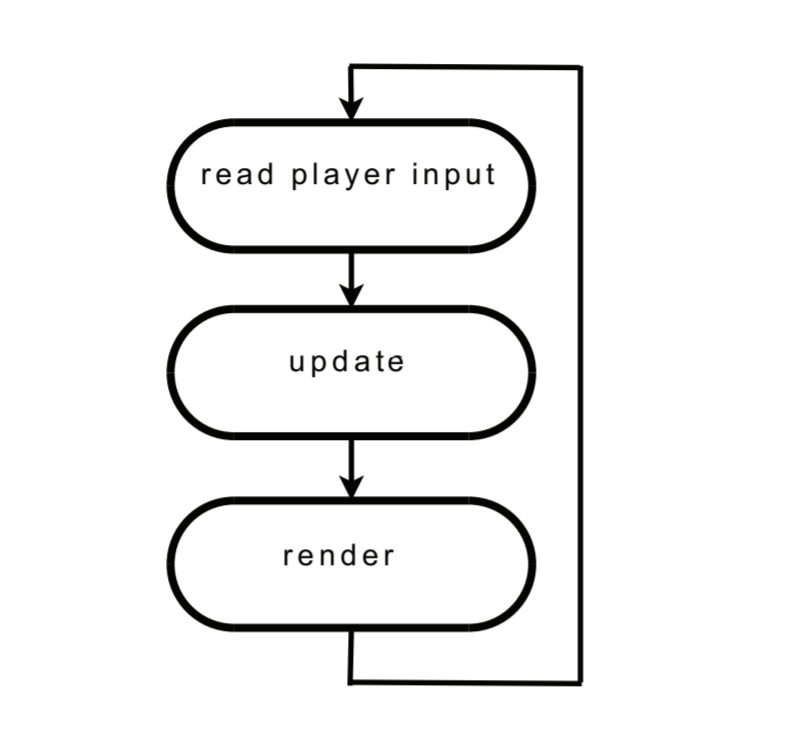
\includegraphics[width=\linewidth,height=5cm]{src/hci2020-images/CoupledGameLoop.png}
        \caption{Coupled Model}
        \label{fig:coupledModel}
    \end{minipage}%
    \begin{minipage}{.5\textwidth}
        \centering
        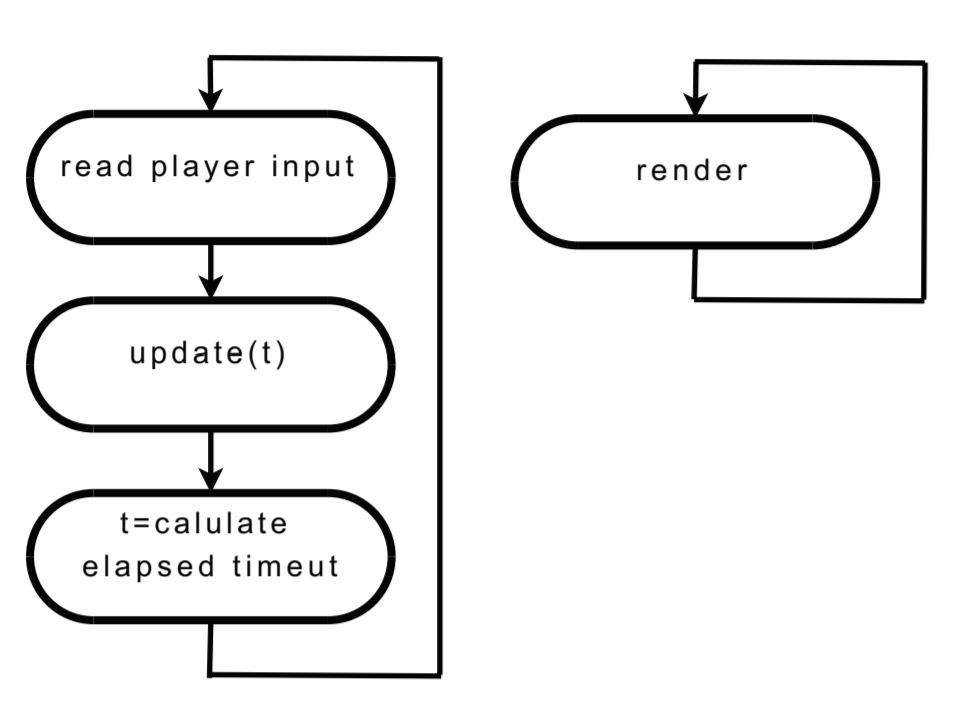
\includegraphics[width=\linewidth,height=5cm]{src/hci2020-images/UncoupledGameLoop.png}
        \caption{Multi-thread Uncoupled Model}
        \label{fig:uncoupledModel}
    \end{minipage}
\end{figure}


\section{Game architectures}
% TODO: What is a game architecture?
Games are a  software product, therefore the  architecture of a game is comparable to that of software and defines how the game is built. Usually, it is not apparent to the player, except for performance \cite{croft_2004}.

According to \cite{mcshaffry_2009}, it is possible to classify any sub-system in a game in one of the three categories: the application layer, the logic layer, and the game view layer. The first layer deals with the operating system and hardware. The second layer manages the game state and how it changes over time. The game view layer presents the current game state with the graphics and sound outputs.

\begin{figure}[!h]
    \centering
    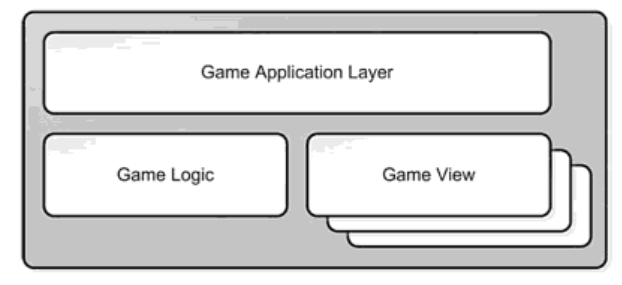
\includegraphics[scale=1.1]{src/GameArchitecture.png}
    \caption{High-level game architecture according to \cite{mcshaffry_2009}}
\end{figure}

Game engines provide \textit{"software that is extensible and can be used as the foundation for many different games without major modification"} \cite{gregory_2019}, and as such, they encapsulate the general game architecture (see figure \ref{fig:Simplified_game_engine}).

\begin{figure}[!h]
    \centering
    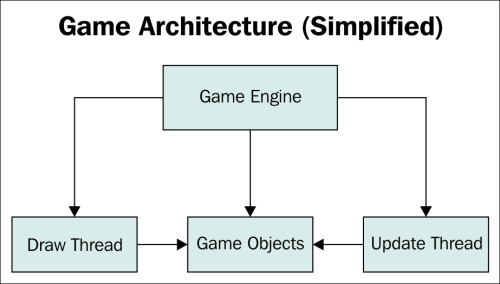
\includegraphics[scale=1.5]{src/hci2020-images/Game_Architecture_Raul_Portales.jpg}
    \caption{Game engine architecture according to \cite{portales}}
    \label{fig:Simplified_game_engine}
\end{figure}

The game engine is responsible for the Update Thread, the Draw Thread and the Game Objects. Each correspond to a general step defined in the general game architecture. The Game Objects are the items the player may or may not interact with during game-play. The Update Thread  is responsible for updating game objects as far as it can whereas the Draw Thread updates all elements visually on the output device \cite{portales}.

% TODO: Objectives of a game architecture?
Game architectures can be updated to better reflect the needs of the game. A well-defined architecture enables better performance and overall results with the final game. In fact, most game engines (as well as the architectures behind it) are crafted for specific platforms and, in some cases, for particular games \cite{gregory_2019}. 


\subsection{Proposed Architecture}
% Our proposal - Two layers
We propose a game architecture based on two layers: 
% Logic layer
one layer handles the game logic whereas the other manages rendering.  The logical layer is CPU-bound and has tasks such as the search for the collectible objects and snake movement. 
% Render layer
The visualization layer involves a shader, a piece of code that runs in the Graphics Processing Unit (GPU), renders all Game Objects on the output device, which includes the collectible objects as well as the snake.

In other words, the logical layer manages the collision and movement of the snake and selects the most promising path given a randomization factor; The visualization layer renders all the elements arranged in the output device, the CPU does not influence these objects.

\section{Render layer}

\subsection{Virtual reality in a inverted sphere}
The illusion in a virtual world and the immersion sense that comes with it require visual material available from all angles. Given that our proposal contemplates a 2D game, the challenge is displaying two-dimensional content in a 3D scenario so that everything happens around the user.

An inverted sphere, a sphere that has only its inner side rendered, makes it possible to fill the entire field of view, it also is the endorsed solution to display equirectangular images in 360 degrees. The procedural generation of a sphere can follow one of the two approaches below:

\begin{enumerate}
  \begin{item} An icosphere, i.e., a sphere which vertices are evenly distributed;
 \end{item}
  \begin{item} Generation of vertices based on longitude/latitude coordinates. \end{item}
\end{enumerate}

For this work, the second approach was adopted due to the possibility of using longitude/latitude as a way to map the UV coordinates through the equation below:

\begin{equation}
R^2 \leftarrow R^3 : (\lambda, \theta) \rightarrow (x, y, z)
\label{equation1}
\end{equation}

% 2 - Mapeamento de UV em uma esfera invertida
To calculate the positions of the sphere vertices, given $N_{latitude}$ latitude values  and $N_{longitude}$ longitude values, the value $R_{longitude}$ is defined as the angular longitude size of a cross-section of the sphere, as seen in the equation \ref{equation1}.

\begin{equation}
R_{longitude} = \frac{2 \pi}{N_{longitude}}
\label{equation1}
\end{equation}

The total angular size of an amount of $i$ of longitude values can be given by the equation \ref{equation2}.

\begin{equation}
\alpha_{i} = i * R_{longitude}
\label{equation2}
\end{equation}

Equations \ref{equation3} and \ref{equation4} define the X and Z positions of sphere points belonging to a cross section of the sphere that has radius $D$.

\begin{equation}
x_{i} = D * \sin(\alpha_{i})
\label{equation3}
\end{equation}

\begin{equation}
z_{i} = D * \cos(\alpha_{i})
\label{equation4}
\end{equation}

In a longitudinal cut, it is possible to notice that the radius $D$ of the cross section is variable along the height of the sphere. It is then determined a value $R$ as the angular size of a latitude value of the sphere, as seen in the equation \ref{equation5}.

\begin{equation}
R_{latitude} = \frac{\pi}{ N_{latitude}}
\label{equation5}
\end{equation}

The total angular size of an amount of $i$ of latitude values can be given by the equation \ref{equation6}.

\begin{equation}
\alpha_{latitude} = i * R_{latitude}
\label{equation6}
\end{equation}

The Y position of the sphere points, considering unit radius, can be given by the equation \ref{equation7}.
\begin{equation}
y_{i} = \cos(\alpha_{latitude})
\label{equation7}
\end{equation}

The radius $D_{yi}$ obtained in a cross section at latitude $i$ is defined in the equation \ref{equation8} as:
\begin{equation}
D_{yi} = 2 * \sin(\alpha_{yi})
\label{equation8}
\end{equation}

By applying the equation \ref{equation8} in the equations \ref{equation3} and ref{equation4} the X and Z positions of the sphere vertices are obtained according to their longitude and latitude coordinates.

\begin{equation}
x_{i} = 2 * \sin(\alpha_{latitude}) * \sin(\alpha_{longitude})
\label{equation9}
\end{equation}

\begin{equation}
z_{i} = 2 * \sin(\alpha_{latitude}) * \cos(\alpha_{longitude})
\label{equation10}
\end{equation}

\section{Logic layer}

\subsection{Managing Game Objects}

\subsection{Snake movement agent} \label{sec:agent}
The movement of the snake is managed by a state evaluation function that analyzes each possible action at any given time. In essence, the serpent is always seeking  the collectible objects, so it evaluates the shortest distance course in the X and Y axes in UV space and, provided that there is no possibility of hitting itself, proceeds through this path and repeats the process. The function below illustrates this procedure:

\begin{equation}
F(A) = R * (D + O)
\label{equation11}
\end{equation}

Where \textit{R} is a randomization factor; \textit{D} represents the \textit{Manhattan} distance between the current position and the collectable object; And \textit{O} is a value attributed to the existence or not of obstacles in this path.

\section{Experiments and Results}
The Snake game was developed for virtual reality in the Unity engine. Figure\ref{fig:VRPerformanceChart}  below illustrates the frame rate in the GearVR through the Oculus performance assessment tool, the \textit{OVR Metrics Tool}:

\begin{figure}[h] 
\centering
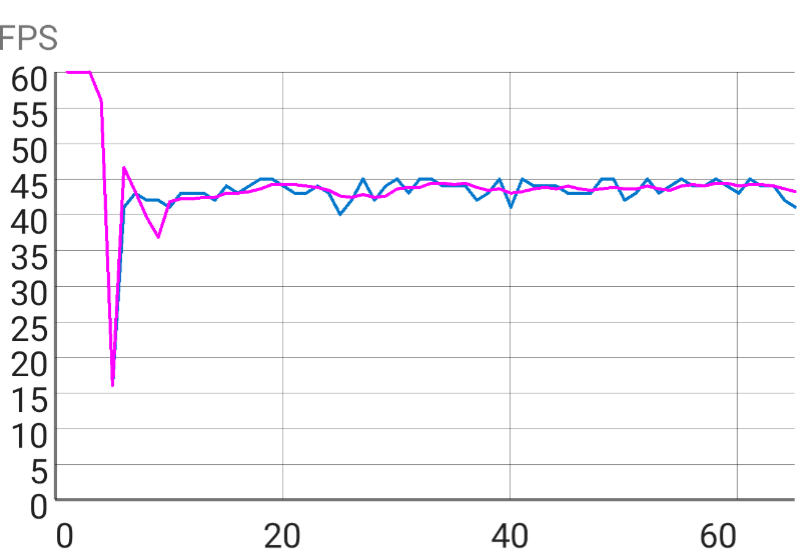
\includegraphics[width=\textwidth]{src/hci2020-images/VRPerformance.png}s
\caption{Frames-per-second recored by the OVR Metrics Tool}
\label{fig:VRPerformanceChart}
\end{figure}

The application presented an average frame-rate of 43.96 fps (frames-per-second), with a minimum of 16 fps and maximum of 60 fps. As represented by the figure \ref{fig:VRPerformanceChart}, the application does not maintain 60 fps and this is mainly due to the garbage collector and the need for GPU code optimization.

% TODO: Define metrics to evaluate architectures
% TODO: Experiment with normal game
% TODO: Experiment with shader-based game
% TODO: Experiment with VR shader-based game
% TODO: Experiment with shader-based game with Raymarching

\section{Conclusions}
We believe it is possible to explore the GPU for additional performance of virtual reality games in mobile devices. For the full paper, we intend to implement the game using the defined architecture and compare results using frames-per-second as the evaluation metric. We also see an opportunity for a full GPU implementation using ray-marching in a 3D environment.
%
% ---- Bibliography ----
%
% BibTeX users should specify bibliography style 'splncs04'.
% References will then be sorted and formatted in the correct style.
%
\bibliographystyle{splncs04}
\bibliography{shaderbasedarch}
\end{document}
